% CMPT 415 Midterm Report -- Executive Summary
% Compile: tectonic midterm_report_executive.tex
\documentclass[11pt,a4paper]{article}

\usepackage[utf8]{inputenc}
\usepackage[T1]{fontenc}
\usepackage{lmodern}
\usepackage[margin=1in]{geometry}
\usepackage{graphicx}
\usepackage{booktabs}
\usepackage{array}
\usepackage{float}
\usepackage{hyperref}
\usepackage{amsmath}
\usepackage{enumitem}
\usepackage{xcolor}
\usepackage{mdframed}

\hypersetup{
    colorlinks=true,
    linkcolor=blue!70!black,
    urlcolor=blue!70!black,
}

\graphicspath{{../artifacts/visualizations/}}

\title{%
  \textbf{CMPT 415 Midterm Report}\\[4pt]
  \Large AI Fairness Dashboard: Executive Summary\\[2pt]
  \normalsize Bias Detection, Qualitative Analysis, and LLM Benchmarking in Lending Domains
}
\author{Siddhant Jain \and Ayaan Lalani}
\date{\today}

\begin{document}
\maketitle
\thispagestyle{plain}

% ===================================================================
\section*{Problem and Motivation}

Lending models trained on historical data can encode systemic biases, leading to
disparate outcomes across protected groups (sex, age, race). Regulatory mandates
(ECOA, EU AI Act) require auditing, but no single metric suffices. This project
has two major goals: (1) define a \textbf{reference audit specification} (the
metrics and response elements an audit must provide to support remediation), and
(2) benchmark our pipeline against \textbf{multiple LLMs} to see where it stands
in the general scheme of things. We build an end-to-end pipeline from raw data
to actionable recommendations and compare it with an LLM-based auditor (Gemini
first; more LLMs planned).

\paragraph{Interim problem statement.}
We focus on evaluating biases in datasets and, over time, in data used by AI
models, to provide recommendations that eliminate those biases from future
systems. Lending is the current domain; the framing applies to any domain where
biased data or models cause unfair outcomes.

% ===================================================================
\section*{What We Built}

A six-step automated pipeline:
\texttt{clean} $\to$ \texttt{train} $\to$ \texttt{fairness} $\to$
\texttt{qualitative} $\to$ \texttt{llm\_benchmark} $\to$ \texttt{visualize}.

\begin{itemize}[nosep, leftmargin=*]
  \item \textbf{Fairness metrics (AIF360):} Disparate Impact (DI), Demographic
        Parity Difference (DPD), Equal Opportunity Difference (EOD), Average
        Odds Difference (AOD), Theil Index. Severity thresholds: Critical
        (DI$<$0.72), High (0.72--0.80), Moderate (0.80--0.95), Low ($\geq$0.95).
  \item \textbf{Qualitative engine:} detects data imbalance, identifies proxy
        features via correlation analysis, maps metric patterns to root causes,
        and recommends specific AIF360 mitigation algorithms.
  \item \textbf{Reference audit specification:} we define the minimum metrics
        (DI, DPD, EOD, AOD, Theil) and response elements (per-group breakdown,
        severity, root causes, concrete recommendations) required for
        remediation-ready analysis.
  \item \textbf{LLM benchmark (Gemini 2.5 Flash; more LLMs planned):}
        independently computes the same metrics using only raw prediction data
        and fairlearn definitions. Zero access to our calculations. Cost:
        \$0.004 total for both datasets.
\end{itemize}

% ===================================================================
\section*{Datasets}

\begin{center}
\small
\begin{tabular}{lcccc}
\toprule
\textbf{Dataset} & \textbf{Records} & \textbf{Protected Attrs} & \textbf{Target} & \textbf{\% Fav.} \\
\midrule
German Credit (UCI) & 1,000 & Sex, AgeGroup, Foreign Worker & Credit approval & 70\% \\
HMDA Georgia (2022) & 6,525 & Race, Sex, Age Group & Loan origination & 72\% \\
\bottomrule
\end{tabular}
\end{center}

% ===================================================================
\section*{Key Results}

\paragraph{German Credit.} All three attributes show \textbf{Moderate} bias
(DI: 0.82--0.94). Sex disadvantages females by 11.5 pp in selection rate; Age
disadvantages under-40 borrowers by 15.9 pp. Both are driven by proxy features
(Age corr.\ $r{=}{-}0.84$) and historical label bias in ground-truth data.
Foreign Worker metrics are statistically unreliable (only 6 non-foreign records).

\paragraph{HMDA.} Race shows Moderate bias (DI = 0.90), with a 41 pp gap
between Asian and Multiracial applicants; representation is severely skewed
(White: 1,252 vs.\ Pacific Islander: 5). Sex is borderline Moderate (DI =
0.93). Age group is effectively fair (DI = 1.01).

\begin{figure}[H]
\centering
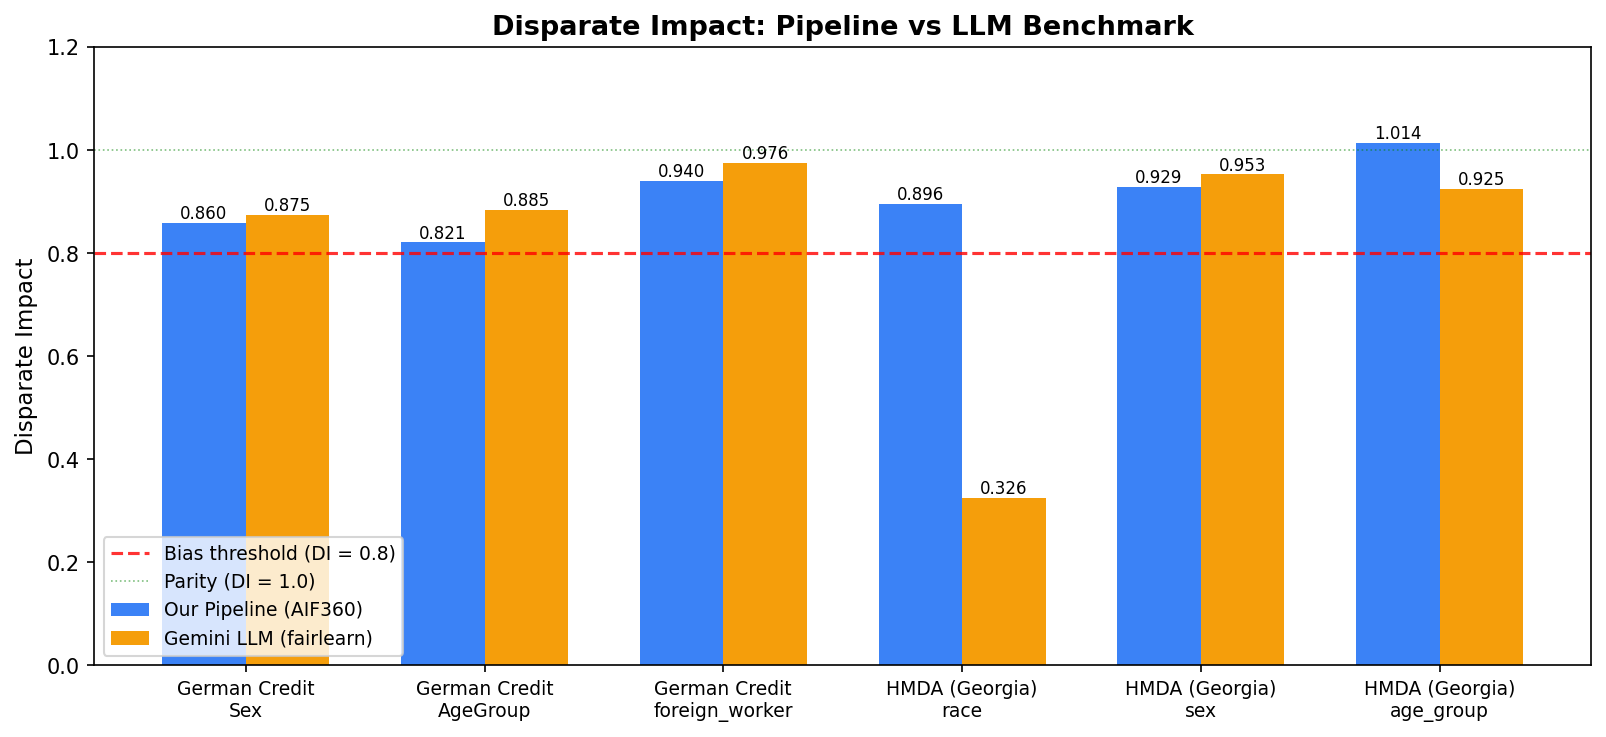
\includegraphics[width=\textwidth]{di_overview.png}
\caption{Disparate Impact across all datasets and attributes (pipeline vs.\ LLM).
         Dashed line marks the 0.8 adverse-impact threshold.}
\end{figure}

% ===================================================================
\section*{Pipeline vs.\ LLM: Agreements and Divergences}

Both approaches agreed on severity for \textbf{4 of 6} attribute-dataset pairs.
The key divergence: on HMDA Race, our pipeline reports DI = 0.90 (Moderate)
while Gemini reports DI = 0.33 (Critical). Gemini selected the American Indian
subgroup ($n{=}10$) as the sole unprivileged baseline; our pipeline uses a
weighted average across all groups. With only 10 records, Gemini's DI is
statistically unreliable, illustrating a fundamental limitation: \textbf{LLMs
lack statistical reasoning about sample sizes.}

\begin{center}
\small
\begin{tabular}{llccc}
\toprule
\textbf{Dataset} & \textbf{Attribute} & \textbf{Ours} & \textbf{Gemini} & \textbf{Agree?} \\
\midrule
German Credit & Sex          & Moderate & Moderate & Yes \\
              & AgeGroup     & Moderate & Moderate & Yes \\
              & Foreign Wkr  & Moderate & Low      & No  \\
\midrule
HMDA          & Race         & Moderate & Critical & No  \\
              & Sex          & Moderate & Low      & No  \\
              & Age Group    & Low      & Low      & Yes \\
\bottomrule
\end{tabular}
\end{center}

\paragraph{LLM strengths.} Richer natural-language explanations; identified
context-specific proxy risks (e.g., zip code as race proxy). \textbf{Cost:
\$0.004 for both datasets combined} -- economically viable for routine audits.

\paragraph{Pipeline strengths.} Fully reproducible; flags small groups
($n<30$) as unreliable; tailors mitigations to detected root causes rather than
repeating generic recommendations.

% ===================================================================
\section*{Top Recommendations by Dataset}

\begin{itemize}[nosep, leftmargin=*]
  \item \textbf{German Credit / Sex:} Apply Disparate Impact Remover
        (preprocessing) and Prejudice Remover (in-processing) to reduce
        correlation between Sex feature and model decisions.
  \item \textbf{German Credit / AgeGroup:} Apply Reweighing to compensate for
        historical label bias; use Equalized Odds post-processing for threshold
        calibration.
  \item \textbf{HMDA / Race:} Collect more data from underrepresented groups;
        apply Reweighing. Treat metrics for groups with $n<30$ as unreliable.
  \item \textbf{HMDA / Sex:} Calibrated Equalized Odds post-processing is a
        low-impact first intervention.
\end{itemize}

% ===================================================================
\section*{What is Next}

\begin{enumerate}[nosep, leftmargin=*]
  \item \textbf{Formalize the reference audit specification} so that other
        tools and LLMs can be evaluated against the same target.
  \item \textbf{Benchmark against additional LLMs} (e.g., Claude, GPT-4,
        open-weight models) on the same data and prompt to see where our
        pipeline stands in the general landscape.
  \item Implement and evaluate the recommended mitigations and measure
        accuracy-fairness trade-offs; add intersectional analysis and more
        lending datasets; build longitudinal fairness monitoring.
\end{enumerate}

\end{document}
